\documentclass{beamer}

\usepackage{amssymb}
\usepackage{latexsym}
\usepackage{amsmath}
\usepackage{amsfonts}
\usepackage{graphicx}
\usepackage{epstopdf}
\usepackage{color} %% to use color: \textcolor{color}{words to be in color} 



\newcommand{\C}{\mathbb C }
\newcommand{\R}{\mathbb R}
\newcommand{\Z}{\mathbb Z}
\newcommand{\G}{\mathcal G}


\title{A Necessary and Sufficient Condition for The Riemann Hypothesis}

\date{\today}

\begin{document}

\frame{\titlepage}


\section{Brief History}

\frame
{
\frametitle{Notations and preliminaries}

Denote $z = x + iy \in \C$.\\

Gamma Function:
\begin{align*}
\Gamma(z) = \int^{\infty}_{0} t^{z-1}e^{-t} dt, x > 0.
\end{align*}

\begin{figure} 
\centering 
\includegraphics[scale=0.25]{pics/GammaAbs.pdf}
\caption{$|\Gamma(z)|$, $-4 < x < 4$} 
\label{fig1} 
\end{figure} 


}

\frame
{
It's known that $\Gamma$ can be extended to a meromorphic function on $\C$ with
simple poles at $0, -1, -2, -3\ldots$.

Later we will use the fact that :\\
$\Gamma(1-z)$ has simple poles at z = 1, 2, \ldots ; the residue of $\Gamma(1-z)$ at $z = k$ is
equal to
\begin{align*}
\frac{(-1)^{k-1}}{(k-1)!}.
\end{align*}
}

%%%%%%%%%%%%%%%%%%%%%%%%%%%%%%%%%%%%%
%Extend through Eular prodcut:
%\begin{align*}
%&\frac{1}{\Gamma(z)} = z e^{rs}\prod^{\infty}_{n=1}(1 + \frac{z}{n})e^{-\frac{s}{n}}, \\
%&r (= \lim_{n \rightarrow \infty}(1 + \frac{1}{2} + \cdots + \frac{1}{n} - ln(n)) \mbox{is the Euler-Mascheroni constant.} 
%\end{align*}
%%%%%%%%%%%%%%%%%%%%%%%%%%%%%%%%%%%%%


\frame
{
The Riemann zeta-function $\zeta(z)$ has its origin in the following identity:

\begin{align*}
\sum^{\infty}_{n=1} \frac{1}{n^z} = \zeta(z) = \prod_{p} (1 - \frac{1}{p^z})^{-1}, x > 1
\end{align*}

By this equation, we know that $\forall \delta > 0$, there exists a number $B(\delta) > 0$, such
that if $x > 1 + \delta$, $|\zeta(z)| < B(\delta)$.

}

\frame
{
\begin{align*}
\frac{1}{\zeta(z)} = \prod_{p} (1 - \frac{1}{p^z})  
                                  = \sum^{\infty}_{n=1} \frac{\mu(n)}{n^z},  x > 1,
\end{align*}

where $\mu$ is m\"obius function, defined as
\begin{align*}
\mu(n) = \Bigg \{\begin{array}{ cc}
      1&           n =1 \\
       (-1)^k &  \mbox{ if $n$ is the product of $k$ different primes} \\
       0 & \mbox{otherwise}
      \end{array}
\end{align*}
}

\frame
{
\begin{center}
\includegraphics[scale=0.3]{pics/Riemann1.pdf}
\end{center}
}

\frame
{
\begin{center}
\includegraphics[scale=0.1]{pics/Riemann.pdf}
\end{center}
In the paper \textbf{On the Number of Primes Less Than a Given Magnitude}(1859), 
Bernhard Riemann extend the function $\zeta(z)$ to all complex values of 
$z$ different from 1, and give the following functional equation
}

\frame
{
\begin{align*}
\zeta(z) = 2^{z}\pi^{z-1}sin(\frac{1}{2}z\pi)\Gamma(1-z)\zeta(1-z),  \forall z \in \C.
\end{align*}

Because $\sin(\frac{1}{2}z\pi)$ has zero at $-2, -4, -6,\ldots$, $\zeta(z)$ has zero at the 
negative even integers. These are called the \textbf{trivial zeros}. \\

Let
\begin{align*}
\xi(z) &= \frac{1}{2}z(z-1)\pi^{-\frac{1}{2}z}\Gamma(\frac{1}{2}z)\zeta(z), \\
\Xi(z) &= \xi(\frac{1}{2} + iz).
\end{align*}
The function equation can be write as $\Xi(z) = \Xi(-z)$.
}


\frame
{
In the very same paper, Riemann states the \textbf{Riemann hypothesis} in terms
of roots of $\Xi(z)$:\\
\textbf{......it is very probable that all roots are real. Of course one would wish for a stricter proof here; 
I have for the time being, after some fleeting futile attempts, provisionally put aside the search for this, 
as it appears unnecessary for the next objective of my investigation.}

\begin{center}
\textcolor{red}{ \Large \textbf{Riemann hypothesis}}

\textcolor{red}{\Large All (nontrival) zero of $\zeta(z)$ have real part $\frac{1}{2}$.}
\end{center}
}


%\frame
{
%\includegraphics[scale=0.3]{try.eps}
}

%\frame
%{ Denote $z = x + iy \in \C$.\\

%Let $f(z) = \frac{z}{e^{z} -1} + \frac{1}{2}z$. It's direct to varify that 

%\begin{align*}
%f(-z) = f(z)
%\end{align*}

%Let $C_k(k = 0, 1, 2 \ldots)$ given by

%\begin{align*}
%f(z) = \frac{z}{e^{z} -1} + \frac{1}{2}z = \sum^{\infty}_{k = 0} C_k z^{2k}.
%\end{align*}
%}

\section{A Necessary and Sufficient Condition for Riemann Hypothesis}
\frame
{
\frametitle{A Necessary and Sufficient Condition for RH}

Bernoulli's number $B_k$ is given by:

\begin{align*}
\frac{z}{e^{z} -1} + \frac{1}{2}z =  1 + B_1\frac{z^{2}}{2!} - B_2 \frac{z^{4}}{4!} + \cdots. \\
\zeta(2k) = 2^{2k -1}\pi^{2k}\frac{B_k}{(2k)!}(k = 1, 2, \ldots). 
\end{align*}

\begin{align*}
A_k = \frac{(2\pi)^{2}}{(2k+2)(2k+1)} \frac{B_{k+1}}{B_k} = \frac{\zeta(2k+2)}{\zeta(2k)}.
\end{align*}
}

\frame
{
Write 
\begin{align*}
f(t) = \sum^{\infty}_{k = 1} \frac{(-1)^{k-1}A_k}{(k-1)!}t^{k}.
\end{align*}

The Riemann Hypothesis is equivalent to the following statement:\\

For any $\epsilon > 0 $, there exists a constant $C(\epsilon) > 0$ such that for any $t > 1$, 
%actually only need a a \in R, t >a the following hold
\begin{align*}
|f(t)| \leq C(\epsilon) t^{\frac{1}{4} + \epsilon}  .
\end{align*}
}

\frame
{
For $c  \in \R$, $ c \notin \Z$ and $t > 0$ define
\begin{align*}
I(c,t) = \frac{1}{2\pi i} \int^{c + \infty}_{c -\infty} \frac{\zeta(2z +2)\Gamma(1-z)}{\zeta(2z)}t^{z} dz.
\end{align*}

Notice if $c > \frac{1}{2}$, and $c \neq 1, 2, \ldots$, then the integrand is analytic on the line $x = c$.

We first show that for $\frac{1}{2} < c < 1$,
\begin{align*}
I(c, t)  =  I(m+\frac{1}{2}, t) + \sum_{1 \leq k \leq m} \frac{(-1)^{k-1}A_{k}}{(k-1)!} t^k.
\end{align*}

}

\frame
{
Consider the contour:
\begin{center}
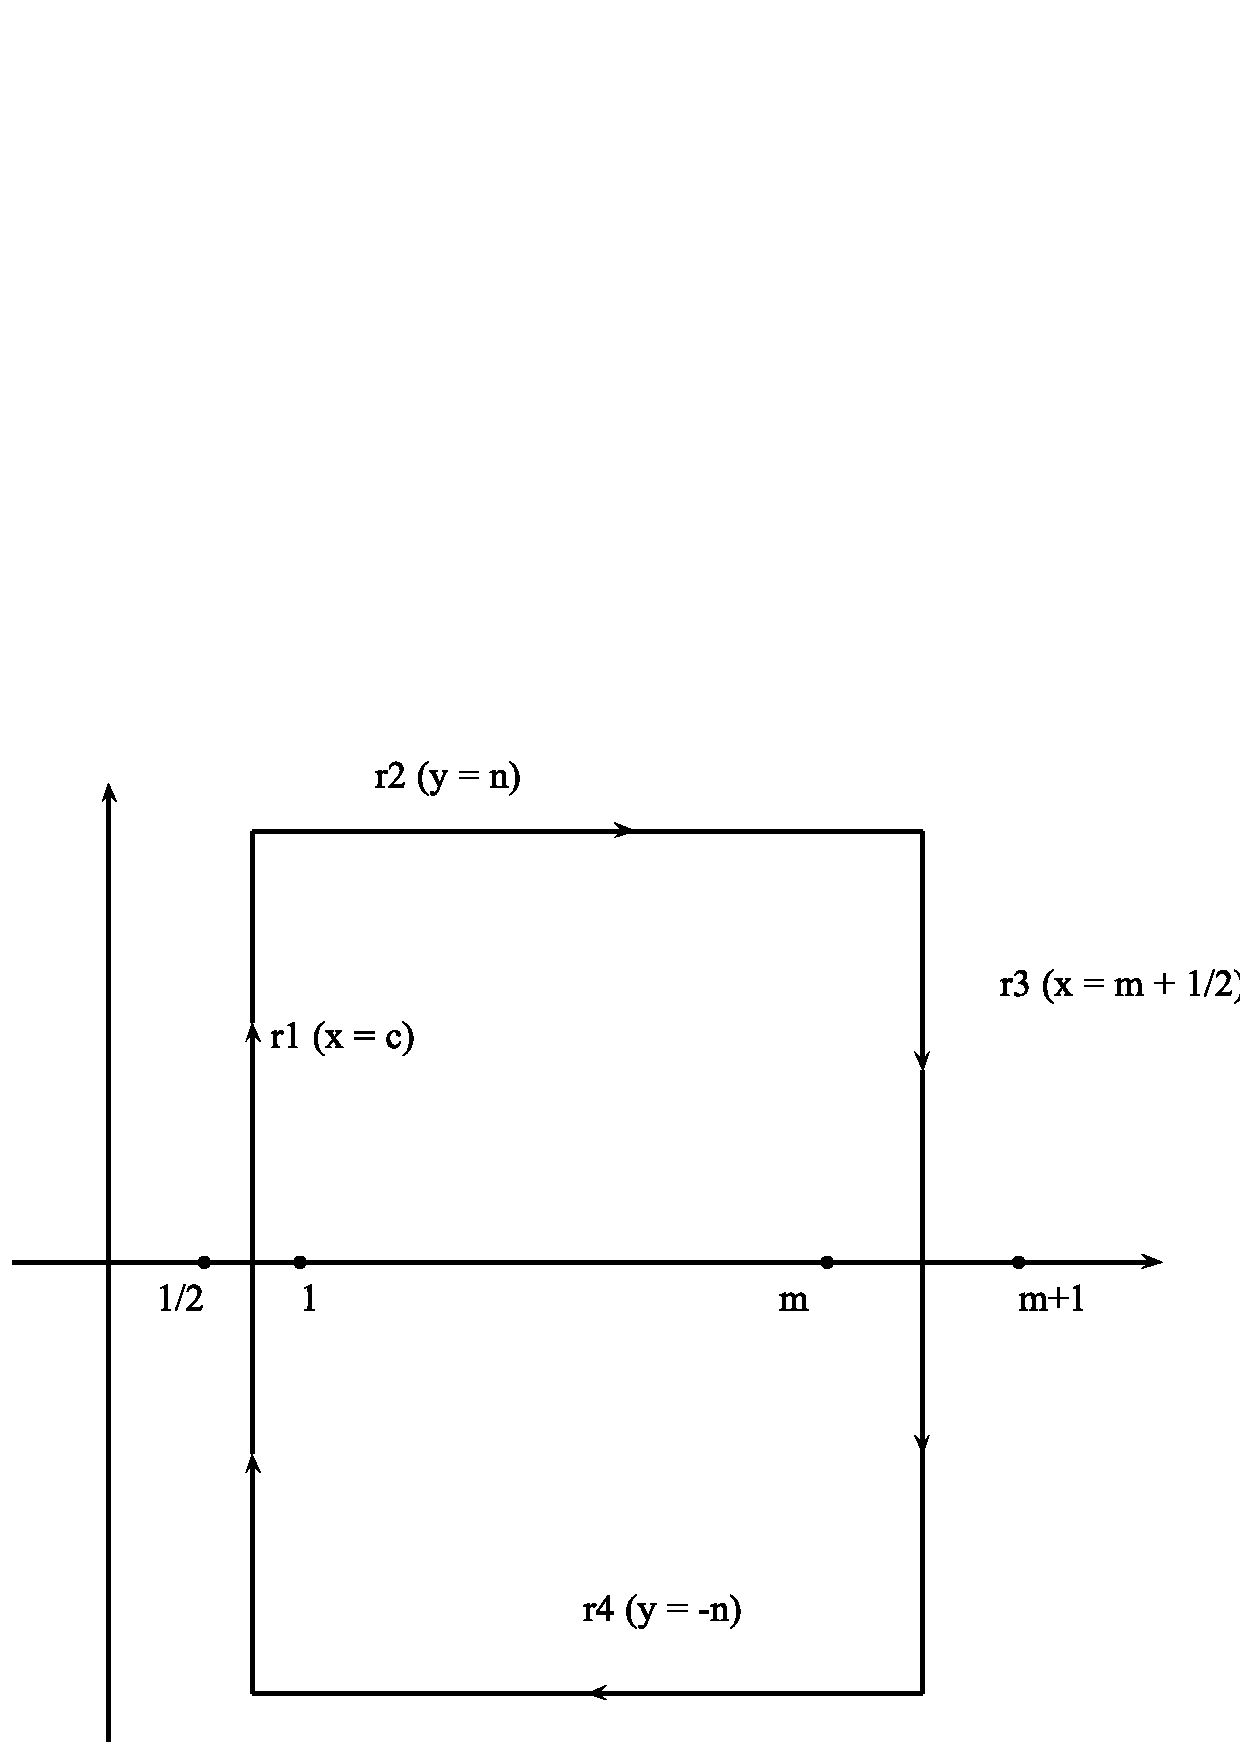
\includegraphics[scale=0.3]{pics/contour.pdf}
\end{center}

We only need to show that 
\begin{align*}
 &\lim_{n \rightarrow \infty} \int_{c + i n}^{m+ \frac{1}{2} + i n} \frac{\zeta(2z +2)\Gamma(1-z)}{\zeta(2z)}t^{z} dz \\
 &=  \lim_{n \rightarrow \infty} \int_{c - i n}^{m+ \frac{1}{2} - i n} \frac{\zeta(2z +2)\Gamma(1-z)}{\zeta(2z)}t^{z} dz = 0
\end{align*}

}

\frame
{
Notice that there exists a constant $C_1$ such that 
\begin{align*}
\left|\frac{\zeta(2z + 2)}{\zeta(2z)} \right| < C_1 \mbox{, $x \geq c$.}
\end{align*}

Also for $ c \leq x \leq m + \frac{1}{2}$, $|t^z| \leq max\{1, |t|^{m+ \frac{1}{2}} \}$.

For $x > \frac{1}{4}, |y| \geq 1$, there exists a constant $C_2$ such that 
\begin{align*}
|\Gamma(1-z)| \leq C_2 e^{\frac{-\pi}{2}|y|} .
\end{align*}
}

\frame
{
On r1( or r4), 

\begin{align*}
\left|\frac{\zeta(2z +2)\Gamma(1-z)}{\zeta(2z)}t^{z} \right| \leq C_1 C_2 max\{1, |t|^{m+ \frac{1}{2}} \} e^{\frac{-\pi}{2}n}.
\end{align*}

\begin{align*}
 &\lim_{n \rightarrow \infty} \left|\int_{c + i n}^{m+ \frac{1}{2} + i n} \frac{\zeta(2z +2)\Gamma(1-z)}{\zeta(2z)}t^{z} dz \right| \\
& \leq \lim_{n \rightarrow \infty}  C_1 C_2 max\{1, |t|^{m+ \frac{1}{2}} \} e^{\frac{-\pi}{2}n}
\int_{c }^{m+ \frac{1}{2} }  dx = 0
\end{align*}

}

\frame
{

On $x = m + \frac{1}{2}$, there is a constant $C_3$ such that  
\begin{align*}
|\Gamma(1-z)| \leq \frac{C_3}{(m-1)!} e^{-(\frac{\pi}{2})|y|}.
\end{align*}

Then by Stirling's formula: 
\begin{align*}
(m-1)! \approx \sqrt{2\pi (m-1)} (\frac{m-1}{e})^{(m-1)}.
\end{align*}

\begin{align*}
\lim_{m \rightarrow \infty} \left|I(m + \frac{1}{2}, t) \right| \leq \lim_{m \rightarrow \infty} \frac{ C_1 C_3 t^{m + \frac{1}{2}}}{(m-1)!}
\int_{- \infty}^{\infty} e^{\frac{-\pi}{2} |y|} dy = 0.
\end{align*}
}

\frame
{
By letting $m \rightarrow \infty$, for any $\frac{1}{2} < c < 1$, $ t > 0$,
\begin{align*}
I(c, t) = \sum^{\infty}_{k = 1} \frac{(-1)^{k-1}A_k}{(k-1)!}t^{k} = f(t).
\end{align*}

Assume now that Riemann Hypothesis is true, then we know that for any $\epsilon > 0$, $\frac{\zeta(2z +2)\Gamma(1-z)}{\zeta(2z)}t^{z}$ is
analytic for $\frac{1}{4} + \epsilon \leq x < 1$.

Furthermore, for any $\epsilon > 0$, there is a $C_1(\epsilon) > 0$ such
that if $x \geq \frac{1}{4} + \epsilon$,
\begin{align*}
\frac{1}{|\zeta(2z)|} \leq C_1 (\epsilon)(1+y^2) .
\end{align*}
}

\frame
{
Similarly, we have 
\begin{align*}
|f(t)| &=  \left|I(\frac{1}{4} + \epsilon, t) \right|\\
            &= \left|\frac{1}{2\pi i} \int^{\frac{1}{4} + \epsilon + \infty}_{\frac{1}{4} + \epsilon -\infty} 
            \frac{\zeta(2z +2)\Gamma(1-z)}{\zeta(2z)}t^{z} dz \right| \\
            &\leq \frac{C_1(\frac{\epsilon}{2})C_2  \zeta(2) t^{\frac{1}{4} + \epsilon} }{2\pi} \int^{+\infty}_{-\infty} (1+y^{2})e^{-\frac{\pi}{2} |y|} dy.
\end{align*}

}

\frame
{
\frametitle{Mellin Transform}
 
If $F(z)$ is analytic for $\frac{1}{2} < x < 1$, and if it tends to zero uniformly with increasing $y$  for 
any real value $c$ between $\frac{1}{2}$ and $1$, with its integral along such a line converging absolutely,
then if for $t > 0$, $\frac{1}{2} < c < 1$,
\begin{align*}
f(t) = \frac{1}{2\pi i} \int^{c + i \infty}_{c - i\infty} F(z)t^{z} dz, 
\end{align*}
we have that 
\begin{align*}
F(z) = \int^{\infty}_{0} f(t)t^{-z-1} dt.
\end{align*}
}

\frame
{For any $\epsilon > 0$, $\frac{1}{2}  + \epsilon < x < 1$, 
\begin{align*}
\left|\frac{\zeta(2z + 2)\Gamma(1-z)}{\zeta(2z)}\right| < C_1 C_2 e^{-\frac{\pi}{2}|y|}.
\end{align*}

By Mellin's transform, for all $\frac{1}{2} < x < 1$,
\begin{align*}
\frac{\zeta(2z + 2)\Gamma(1-z)}{\zeta(2z)} &= \int^{\infty}_{0} f(t) t^{-z -1} dt \\
                                                                                       &= \int^{1}_{0} f(t) t^{-z -1} dt + \int^{\infty}_{1} f(t) t^{-z -1} dt\\
                                                                                       &= I_1 + I_2
\end{align*}

}

\frame
{
Since $f(t) = O(t)$ as $t \rightarrow 0^+$,  for any $0 < x < 1 $,  there exists a constant $C_4(x)$ such that
\begin{align*}
|I_1| &\leq \int^{1}_{0} |f(t) t^{-z -1}| dt \\
            &\leq  C_4(x)\int^{1}_{0} t^{-x} dt  < + \infty.
\end{align*} 
}

\frame
{
If for any $\epsilon > 0$, there is a constant $C(\epsilon)$ such that
\begin{align*}
|f(t)| \leq C(\epsilon) t^{\frac{1}{4} + \epsilon} \mbox{, } t > 1.
\end{align*}
Assume $\frac{1}{4} < x < 1$, denote $x = \frac{1}{4} + \epsilon$ ($0 < \epsilon < \frac{3}{4})$,
\begin{align*}
|I_2| & \leq \int^{\infty}_{1} |f(t) t^{-z -1}| dt \\
           & \leq C(\frac{\epsilon}{2}) \int^{\infty}_{1} t^{-1-\frac{\epsilon}{2}} dt  < \infty .
\end{align*}
}

\frame
{
Therefore $\int^{\infty}_{0} f(t) t^{-z -1} dt$ converges absolutely and represents an 
analytic function in the strip $\frac{1}{4} < x < 1$. In other words, $\frac{\zeta(2z + 2)\Gamma(1-z)}{\zeta(2z)}$
is an analytic function in this strip. Further, since $\zeta(2z + 2)\Gamma(1-z)$ is analytic and non-vanishing
for $\frac{1}{4} < x < 1$, it follows that $\zeta(2z)$ is analytic and non-vanishing for $\frac{1}{4} < x < 1$.
This implies the Riemann Hypothesis.
} 

\frame
{
\frametitle{A Generalization}

Let $\G$ be the family of functions G of the complex variables $z$ such that $G \in \G$ iff the following hold:
 
  \begin{enumerate}
  \item $G$ is analytic on the half-plane $x > \frac{1}{4}$ and it satisfies
               \begin{align*}
                     |G(z)| \leq \frac{e^{(\frac{\pi}{2})|z|}}{|z|^4}, 
                 \end{align*}      
  \item $G(z) \neq 0$ if $\frac{1}{4} < x < \frac{1}{2}$.
  \end{enumerate}

}

\frame
{ 
\begin{align*}
\Phi_{G}(t) = \sum^{\infty}_{k = 1} \frac{(-1)^{k-1}A_k G(k)}{(k-1)!}t^k.
\end{align*}

Condition (C): For any $\epsilon > 0$, there exists a $C(\epsilon) > 0$ depending on $\epsilon$ such that
\begin{align*}
|\Phi_G (t)| \leq C(\epsilon) t^{\frac{1}{4} + \epsilon}, \mbox{if $x > 1$}.
\end{align*}

\begin{theorem}[A Generalization]
If there exists a function $G \in \G$ satisfying the condition (C), then the Riemann Hypothesis 
is true. Conversely, if the Riemann Hypothsis is true, then Condition (C) is satisfied by any $G \in \G$.
\end{theorem}

}

\end{document}
